\documentclass[a4paper,12pt]{article}
\usepackage[utf8]{inputenc}
\usepackage[vietnamese]{babel}
\usepackage{graphicx}
\usepackage{array}
\usepackage{calc}
\usepackage{float}
\usepackage{enumitem}
\usepackage[T1]{fontenc} % Bắt buộc để hiển thị đúng chữ đ
\usepackage[utf8]{inputenc}
\usepackage{indentfirst}
\usepackage{listings}
\usepackage{xcolor}
\usepackage[table]{xcolor}
\usepackage{fontawesome5}
\usepackage{alltt}
\usepackage{longtable}
\usepackage[T1]{fontenc}
\usepackage{lmodern}
\usepackage{multirow}
\usepackage{booktabs}
\usepackage{placeins}
\usepackage{amsmath}
\usepackage{amssymb}
\usepackage{tabularx}
\usepackage{hyperref}
\usepackage{ragged2e}
\usepackage{pmboxdraw}
\usepackage{fancyhdr}  % Thêm gói để tạo header, footer
\usepackage{titlesec}   % Để thay đổi kích thước của title section
\usepackage{tocloft}    % Để tùy chỉnh table of contents
\usepackage{geometry}
\geometry{a4paper, total={170mm,257mm}, left=20mm, top=20mm}

\pagestyle{fancy}
\fancyhf{}
\fancyhead[L]{\textbf{Báo Cáo IT4788}}
\fancyhead[R]{Nhóm 11}
\fancyfoot[L]{}
\fancyfoot[C]{\thepage}
\fancyfoot[R]{Fresh Fridge}

\setlength{\headheight}{20pt}
\setlength{\footskip}{30pt}

% Định nghĩa màu sắc giống IDE Light Theme
\definecolor{commentgreen}{rgb}{0,0.4,0}
\definecolor{keywordblue}{rgb}{0,0,0.8}
\definecolor{stringred}{rgb}{0.6,0,0}
\definecolor{graynumber}{rgb}{0.5,0.5,0.5}

\lstset{
    backgroundcolor=\color{white},   
    commentstyle=\color{commentgreen},
    keywordstyle=\color{keywordblue}\bfseries,
    numberstyle=\tiny\color{graynumber},
    stringstyle=\color{stringred},
    basicstyle=\ttfamily\small,
    breakatwhitespace=false,         
    breaklines=true,                 
    captionpos=b,                    
    keepspaces=true,                 
    numbers=left,                    
    numbersep=5pt,                  
    showspaces=false,                
    showstringspaces=false,
    showtabs=false,                  
    tabsize=2,
    frame=single,
    rulecolor=\color{black!10},
    % Xử lý tiếng Việt bên trong code
    literate={á}{{\'a}}1 {à}{{\`a}}1 {ả}{{\?a}}1 {ã}{{\~a}}1 {ạ}{{.a}}1
             {é}{{\'e}}1 {è}{{\`e}}1 {ẻ}{{\?e}}1 {ẽ}{{\~e}}1 {ẹ}{{.e}}1
             {í}{{\'i}}1 {ì}{{\`i}}1 {ỉ}{{\?i}}1 {ĩ}{{\~i}}1 {ị}{{.i}}1
             {ó}{{\'o}}1 {ò}{{\`o}}1 {ỏ}{{\?o}}1 {õ}{{\~o}}1 {ọ}{{.o}}1
             {ú}{{\'u}}1 {ù}{{\`u}}1 {ủ}{{\?u}}1 {ũ}{{\~u}}1 {ụ}{{.u}}1
             {ý}{{\'y}}1 {ỳ}{{\`y}}1 {ỷ}{{\?y}}1 {ỹ}{{\~y}}1 {ỵ}{{.y}}1
             {đ}{{\textsubscript{d}}}1
}

% Định nghĩa ngôn ngữ JSON cho listings
\lstdefinelanguage{json}{
    basicstyle=\ttfamily\small,
    numbers=left,
    numberstyle=\tiny\color{graynumber},
    stepnumber=1,
    numbersep=8pt,
    showstringspaces=false,
    breaklines=true,
    frame=single,
    backgroundcolor=\color{white},
    morestring=[b]",
    stringstyle=\color{stringred},
    comment=[l]{:},
    commentstyle=\color{black},
    literate=
     *{0}{{{\color{blue}0}}}{1}
      {1}{{{\color{blue}1}}}{1}
      {2}{{{\color{blue}2}}}{1}
      {3}{{{\color{blue}3}}}{1}
      {4}{{{\color{blue}4}}}{1}
      {5}{{{\color{blue}5}}}{1}
      {6}{{{\color{blue}6}}}{1}
      {7}{{{\color{blue}7}}}{1}
      {8}{{{\color{blue}8}}}{1}
      {9}{{{\color{blue}9}}}{1}
      {:}{{{\color{black}{:}}}}{1}
      {,}{{{\color{black}{,}}}}{1}
      {\{}{{{\color{keywordblue}{\{}}}}{1}
      {\}}{{{\color{keywordblue}{\}}}}}{1}
      {[}{{{\color{keywordblue}{[}}}}{1}
      {]}{{{\color{keywordblue}{]}}}}{1}
}

% Đổi tên tiêu đề danh mục
\renewcommand{\lstlistlistingname}{Danh mục mã nguồn}

% Đổi tên nhãn tại mỗi đoạn code (Ví dụ: Mã nguồn 1: ...)
\renewcommand{\lstlistingname}{Mã nguồn}

\addto\captionsvietnamese{
  \renewcommand{\listfigurename}{Danh mục hình ảnh}
  \renewcommand{\listtablename}{Danh mục bảng biểu}
}
% --- ĐỊNH NGHĨA MÀU SẮC ---
\definecolor{headergreen}{RGB}{198, 239, 206} % Màu xanh nhẹ dịu mắt
\definecolor{headerorange}{RGB}{255, 235, 156} % Màu cam nhạt làm nổi bật tiêu đề cột
\definecolor{graybg}{gray}{0.95}

% --- TĂNG CHIỀU CAO DÒNG ---
\renewcommand{\arraystretch}{1.4} % Giúp bảng không bị bí
\begin{document}

\begin{titlepage}
\begin{center}
    \textbf{\Large ĐẠI HỌC BÁCH KHOA HÀ NỘI}\\[0.5em]
    \textbf{\large TRƯỜNG CÔNG NGHỆ THÔNG TIN \& TRUYỀN THÔNG}

    
\includegraphics[width=0.2\textwidth]{divider.png}\\[2em]

    
\includegraphics[width=0.7\textwidth]{soict.jpg}

    \vspace{1cm}

    \textbf{\Large GVHD: ThS. Nguyễn Mạnh Tuấn,} \\
    \textbf{\Large TS. Nguyễn Quốc Tuấn}
    \\[1em]

    \textbf{\Large Chủ đề thực hiện:}\\[0.5em]
    {\Large \textbf{XÂY DỰNG ỨNG DỤNG ``ĐI CHỢ TIỆN LỢI''}}\\[1em]

    \normalsize
    Mã lớp: \textbf{162304} \hspace{2em}
    Nhóm: \textbf{11} \hspace{2em} \\[1em]

    Môn học: \textbf{Phát triển ứng dụng đa nền tảng} \hspace{0.5em} Mã môn học: \textbf{IT4788}\\[2em]

    \textbf{Các thành viên trong nhóm:}

    \vspace{1em}
    \setlength{\tabcolsep}{6pt} 
    \renewcommand{\arraystretch}{1.3}
    
    \begin{tabular}{|c|p{4cm}|c|p{7cm}|}
        \hline
        % Sử dụng \multicolumn để căn giữa tiêu đề
        \textbf{STT} & \multicolumn{1}{c|}{\textbf{Họ và tên}} & \textbf{MSSV} & \multicolumn{1}{c|}{\textbf{Email}} \\
        \hline
        1 & Nguyễn Thế Anh & 20224921 & anh.nt224921@sis.hust.edu.vn \\ \hline
        2 & Quản Tuấn Huy & 20225014 & huy.qt225014@sis.hust.edu.vn \\ \hline
        3 & Phạm Trung Kiên & 20225026 & kien.pt225026@sis.hust.edu.vn \\ \hline
        4 & Nhữ Ngọc Minh & 20225046 & minh.nn225046@sis.hust.edu.vn \\
        \hline
        5 & Trần Bảo Long & 20225038 & long.tb225038@sis.hust.edu.vn \\ \hline
    \end{tabular}
    \end{center}

\vfill
\begin{center}
    \textit{Hà Nội, tháng 12 năm 2025}
\end{center}

\end{titlepage}

\renewcommand{\abstractname}{Lời nói đầu}
\begin{abstract}
Trong bối cảnh cuộc sống hiện đại ngày càng bận rộn, việc quản lý công việc gia đình, đặc biệt là khâu mua sắm và chuẩn bị bữa ăn hàng ngày, trở thành một thách thức không nhỏ. Việc đi chợ hay siêu thị thường tốn nhiều thời gian và dễ xảy ra tình trạng mua thừa hoặc thiếu thực phẩm. Thêm vào đó, việc không theo dõi sát sao thực phẩm trong tủ lạnh dẫn đến tình trạng lãng phí do hết hạn sử dụng. Nhận thấy nhu cầu thực tế này, chúng tôi đã quyết định xây dựng dự án ``Xây dựng ứng dụng di động đa nền tảng ``Đi chợ tiện lợi'' ''. Ứng dụng này ra đời với mong muốn cung cấp một công cụ hữu ích, giúp người dùng đơn giản hóa và tối ưu hóa các công việc liên quan đến mua sắm và quản lý thực phẩm. 

Đề tài ``Đi chợ tiện lợi'' mang ý nghĩa thiết thực, giải quyết trực tiếp những vấn đề hàng ngày mà nhiều cá nhân và gia đình gặp phải. Ứng dụng không chỉ giúp tiết kiệm thời gian và công sức trong việc mua sắm và nấu nướng mà còn đóng vai trò quan trọng trong việc quản lý chi tiêu và dinh dưỡng hiệu quả hơn. Bằng cách cung cấp các công cụ để theo dõi thực phẩm, lên kế hoạch bữa ăn và nhắc nhở thông minh về hạn sử dụng, ứng dụng góp phần giảm thiểu lãng phí thực phẩm – một vấn đề đang được xã hội quan tâm. Hơn nữa, với tính năng chia sẻ danh sách mua sắm trong gia đình, ứng dụng còn tăng cường sự phối hợp giữa các thành viên, giúp việc mua sắm trở nên khoa học và hiệu quả, từ đó nâng cao chất lượng cuộc sống.
\end{abstract}

\vspace{0.5cm}

\hspace*{10cm}  % Cách mép trái 10cm
\parbox{5cm}{
    \raggedleft
    \textbf{Nhóm 11}
}

\newpage
\tableofcontents
\listoffigures   % Hiển thị Danh mục hình ảnh
\listoftables    % Hiển thị Danh mục bảng biểu
\lstlistoflistings

\newpage
\section*{Phân công thành viên trong nhóm}

\noindent
\begin{table}[H]
    \small % Sử dụng cỡ chữ nhỏ hơn để bảng vừa vặn với lề trang
    \centering
    \renewcommand{\arraystretch}{1.5} % Tăng khoảng cách dòng để dễ đọc
    \setlength{\tabcolsep}{4pt}      % Giảm khoảng cách lề cột để tối ưu không gian
    
    % Định nghĩa độ rộng các cột để tránh chồng lấn:
    % Cột 1: 2.8cm, Cột 2: 4.2cm (tự ngắt dòng), Cột 3: 2.2cm, Cột 4: Tự giãn (X), Cột 5: 1.5cm
    \begin{tabularx}{\textwidth}{|>{\RaggedRight\arraybackslash}p{2.8cm}|>{\RaggedRight\arraybackslash}p{4.2cm}|>{\centering\arraybackslash}p{2.2cm}|X|>{\centering\arraybackslash}p{1.5cm}|}
        \hline
        \rowcolor{gray!20} 
        \textbf{Họ và tên} & \textbf{Email} & \textbf{SĐT} & \textbf{Tổng hợp công việc thực hiện} & \textbf{Đánh giá} \\ \hline
        
        Nguyễn Thế Anh & anh.nt224921@ \newline sis.hust.edu.vn & 0912345xxx & 
        \begin{itemize}[leftmargin=*, nosep, topsep=0pt]
            \item Phát triển Frontend.
            \item Viết báo cáo.
        \end{itemize} & 100\% \\ \hline
        
        Quản Tuấn Huy & huy.qt225014@ \newline sis.hust.edu.vn & 0987654xxx & 
        \begin{itemize}[leftmargin=*, nosep]
            \item Phát triển Frontend.
        \end{itemize} & 100\% \\ \hline
        
        Phạm Trung Kiên & kien.pt225026@ \newline sis.hust.edu.vn & 0901122xxx & 
        \begin{itemize}[leftmargin=*, nosep]
            \item Phân tích yêu cầu.
            \item Viết tài liệu.
        \end{itemize} & 100\% \\ \hline
        
        Nhữ Ngọc Minh & minh.nn225046@ \newline sis.hust.edu.vn & 0933445xxx & 
        \begin{itemize}[leftmargin=*, nosep]
            \item Phát triển Backend.
        \end{itemize} & 100\% \\ \hline
        
        Trần Bảo Long & long.tb225038@ \newline sis.hust.edu.vn & 0977889xxx & 
        \begin{itemize}[leftmargin=*, nosep]
            \item Phát triển Backend.
        \end{itemize} & 100\% \\ \hline
    \end{tabularx}
    \caption{Bảng phân công nhiệm vụ và đánh giá thành viên}
    \label{tab:phan-cong}
\end{table}


\newpage
\section{Khảo sát bài toán}
\subsection{Mô tả yêu cầu bài toán}
Trong cuộc sống hiện đại, người dùng thường gặp khó khăn trong việc quản lý danh sách các mặt hàng cần mua, theo dõi thực phẩm đã có trong tủ lạnh, cũng như lên kế hoạch cho các bữa ăn hàng ngày sao cho tiết kiệm và khoa học. Ứng dụng “Đi chợ tiện lợi” được xây dựng nhằm giải quyết các vấn đề đó bằng cách hỗ trợ người dùng quản lý toàn bộ quy trình mua sắm và tiêu thụ thực phẩm một cách thông minh và hiệu quả. 

Cụ thể, ứng dụng cho phép người dùng tạo và chia sẻ danh sách mua sắm với các thành viên trong gia đình, giúp phối hợp việc mua hàng và tránh trùng lặp. Người dùng có thể lưu trữ thông tin thực phẩm trong tủ lạnh, theo dõi ngày hết hạn và nhận thông báo nhắc nhở khi thực phẩm sắp hỏng. Hệ thống hỗ trợ lên kế hoạch bữa ăn theo ngày hoặc tuần, đồng thời đề xuất món ăn dựa trên các nguyên liệu sẵn có, giúp người dùng tận dụng thực phẩm hiệu quả hơn. 

Ngoài ra, ứng dụng còn cho phép quản lý công thức nấu ăn yêu thích, tìm kiếm và phân loại thực phẩm, cũng như cung cấp báo cáo thống kê về hoạt động mua sắm và tiêu thụ, giúp người dùng theo dõi thói quen chi tiêu và cải thiện chế độ dinh dưỡng. 

Để đảm bảo hoạt động ổn định và đầy đủ chức năng, hệ thống yêu cầu phát triển server lưu trữ dữ liệu, dịch vụ web xử lý yêu cầu từ ứng dụng di động, chức năng quản trị dành cho admin, cũng như giao diện người dùng thân thiện và push notification thông minh. Toàn bộ ứng dụng được phát triển theo hướng đa nền tảng, đảm bảo khả năng sử dụng linh hoạt trên nhiều thiết bị di động khác nhau. 

\subsection{Xác định thông tin cơ bản cho nghiệp vụ của bài toán}
\noindent
\begin{table}[H]
    \small % Giảm cỡ chữ để chứa được nhiều nội dung hơn
    \centering
    \renewcommand{\arraystretch}{1.4}
    \setlength{\tabcolsep}{4pt}
    
    % Sử dụng tabularx để tự động giãn độ rộng các cột
    \begin{tabularx}{\textwidth}{|>{\RaggedRight\arraybackslash}p{3cm}|X|X|X|}
        \hline
        \rowcolor{gray!20} 
        \textbf{Nghiệp vụ} & \textbf{Input} & \textbf{Process} & \textbf{Output} \\ \hline
        
        % Use Case 1
        1. Tạo danh sách mua sắm & 
        \begin{itemize}[leftmargin=*, nosep]
            \item Thực phẩm (tên, số lượng, đơn vị)
            \item Người đảm nhận (trong group)
        \end{itemize} & 
        \begin{itemize}[leftmargin=*, nosep]
            \item Kiểm tra thực đơn gợi ý món
            \item Lưu danh sách vào CSDL
            \item Gửi thông báo
        \end{itemize} & 
        \begin{itemize}[leftmargin=*, nosep]
            \item Danh sách được tạo
            \item Thông báo gửi đi
        \end{itemize} \\ \hline
        
        % Use Case 2
        2. Tạo thực đơn cho bữa ăn & 
        \begin{itemize}[leftmargin=*, nosep]
            \item Ngày/bữa ăn
            \item Danh sách món ăn
            \item Thực phẩm trong bếp
        \end{itemize} & 
        \begin{itemize}[leftmargin=*, nosep]
            \item Gợi ý món phù hợp thực phẩm sẵn có
            \item Lưu thực đơn vào CSDL
        \end{itemize} & 
        \begin{itemize}[leftmargin=*, nosep]
            \item Thực đơn mới
            \item Gợi ý món ăn
        \end{itemize} \\ \hline
        
        % Use Case 3
        3. Thêm thực phẩm vào bếp & 
        \begin{itemize}[leftmargin=*, nosep]
            \item Tên, số lượng, đơn vị
            \item Ngày hết hạn
        \end{itemize} & 
        \begin{itemize}[leftmargin=*, nosep]
            \item Kiểm tra trùng lặp
            \item Nếu trùng $\rightarrow$ chỉnh sửa
            \item Nếu mới $\rightarrow$ lưu CSDL
        \end{itemize} & 
        Thực phẩm mới được thêm vào danh sách bếp \\ \hline
        
        % Use Case 4
        4. Tạo công thức nấu ăn & 
        \begin{itemize}[leftmargin=*, nosep]
            \item Tên món ăn
            \item Nguyên liệu
            \item Người tạo
        \end{itemize} & 
        \begin{itemize}[leftmargin=*, nosep]
            \item Kiểm tra thông tin hợp lệ
            \item Lưu công thức vào CSDL
        \end{itemize} & 
        \begin{itemize}[leftmargin=*, nosep]
            \item Công thức mới được tạo
            \item Sẵn sàng tìm kiếm
        \end{itemize} \\ \hline
        
        % Use Case 5
        5. Tạo thực phẩm & 
        \begin{itemize}[leftmargin=*, nosep]
            \item Tên thực phẩm
            \item Danh mục
        \end{itemize} & 
        \begin{itemize}[leftmargin=*, nosep]
            \item Kiểm tra trùng tên
            \item Lưu vào CSDL cá nhân
        \end{itemize} & 
        Thực phẩm cá nhân được tạo và thêm vào nhóm \\ \hline
    \end{tabularx}
    \caption{Chi tiết luồng xử lý các nghiệp vụ chính của ứng dụng}
    \label{tab:nghiep-vu}
\end{table}

\newpage
\section{Đặc tả yêu cầu bài toán}

\subsection{Giới thiệu chung}
Xác định các tác nhân của hệ thống
\noindent
\begin{table}[H]
    \centering
    \small % Duy trì cỡ chữ nhỏ để đồng bộ với các bảng khác
    \renewcommand{\arraystretch}{1.5} % Tạo khoảng cách dòng thông thoáng
    \setlength{\tabcolsep}{10pt} % Tăng khoảng cách lề cột để dễ quan sát
    
    \begin{tabularx}{\textwidth}{|c|>{\RaggedRight\arraybackslash\bfseries}p{4cm}|X|}
        \hline
        \rowcolor{gray!20} 
        \textbf{STT} & \textbf{Tên tác nhân} & \textbf{Mô tả tác nhân} \\ \hline
        
        1 & Người dùng & Người sử dụng ứng dụng. \\ \hline
        
        2 & Quản trị viên & Quản trị viên quản lý hệ thống. \\ \hline
    \end{tabularx}
    \caption{Bảng liệt kê và mô tả các tác nhân trong hệ thống}
    \label{tab:tac-nhan}
\end{table}
Xác định các ca sử dụng
\begin{table}[H]
    \centering
    \footnotesize % Sử dụng cỡ chữ nhỏ hơn để chứa được nhiều cột
    \renewcommand{\arraystretch}{1.5}
    \setlength{\tabcolsep}{3pt} % Tối ưu khoảng cách giữa các cột
    
    % Định nghĩa các cột: 
    % STT (c), Mã (c), Tên (p), Mô tả (X - tự giãn), Tác nhân (p), Độ phức tạp (c)
    \begin{tabularx}{\textwidth}{|c|c|>{\RaggedRight\arraybackslash}p{2.5cm}|X|>{\RaggedRight\arraybackslash}p{2.2cm}|c|}
        \hline
        \rowcolor{gray!20} 
        \textbf{STT} & \textbf{Mã UC} & \textbf{Tên Use Case} & \textbf{Mô tả Use Case} & \textbf{Tác nhân} & \textbf{Độ phức tạp} \\ \hline
        
        1 & UC001 & Quản lý danh sách mua sắm & Người dùng tạo, chỉnh sửa, xóa, theo dõi danh sách mặt hàng cần mua. Giao cho người dùng đi chợ. & Người dùng & Cao \\ \hline
        
        2 & UC002 & Quản lý dự định bữa ăn & Người dùng lên kế hoạch bữa ăn theo ngày hoặc tuần. & Người dùng & Cao \\ \hline
        
        3 & UC003 & Quản lý thực phẩm trong bếp & Người dùng nhập, chỉnh sửa, theo dõi thông tin thực phẩm tích trữ (tủ lạnh, bếp). & Người dùng & Thấp \\ \hline
        
        4 & UC004 & Quản lý công thức nấu ăn & Người dùng lưu trữ và quản lý các công thức nấu ăn. & Người dùng, Quản trị viên & Trung bình \\ \hline
        
        5 & UC005 & Quản lý danh sách thực phẩm & Người dùng quản lý danh sách các loại thực phẩm. & Người dùng, Quản trị viên & Trung bình \\ \hline
        
        6 & UC006 & Quản lý nhóm & Người dùng tạo/xóa nhóm, thêm/xóa thành viên trong nhóm. & Người dùng & Thấp \\ \hline
        
        7 & UC007 & Thống kê và báo cáo & Hệ thống tạo báo cáo về mua sắm và tiêu thụ thực phẩm. & Người dùng & Trung bình \\ \hline
        
        8 & UC008 & Quản trị người dùng & Quản trị viên quản lý tài khoản người dùng. & Quản trị viên & Thấp \\ \hline
    \end{tabularx}
    \caption{Bảng tổng hợp danh mục Use Case của hệ thống}
    \label{tab:danh-muc-usecase}
\end{table}
\subsection{Biểu đồ use case}
\subsubsection{Biểu đồ use case tổng quan}
\begin{figure}[H]
    \centering 
    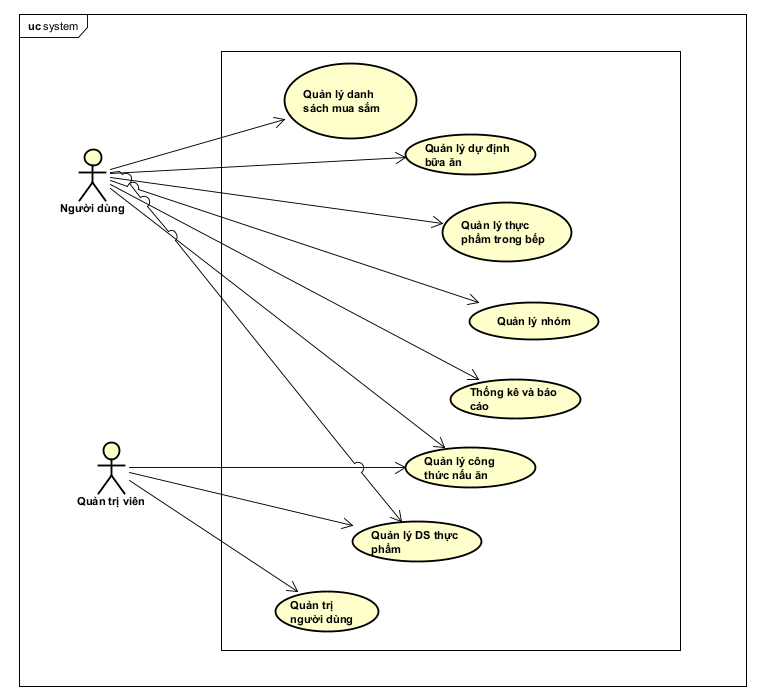
\includegraphics[width=0.9\textwidth]{UC_tong_quan.png}
    \caption{Biểu đồ Use Case tổng quan của hệ thống}
    \label{fig:usecase-tongquan}
\end{figure}
\subsubsection{Biểu đồ use case phân rã mức 2}
\textbf{Quản lý danh sách mua sắm}
\begin{figure}[H]
    \centering
    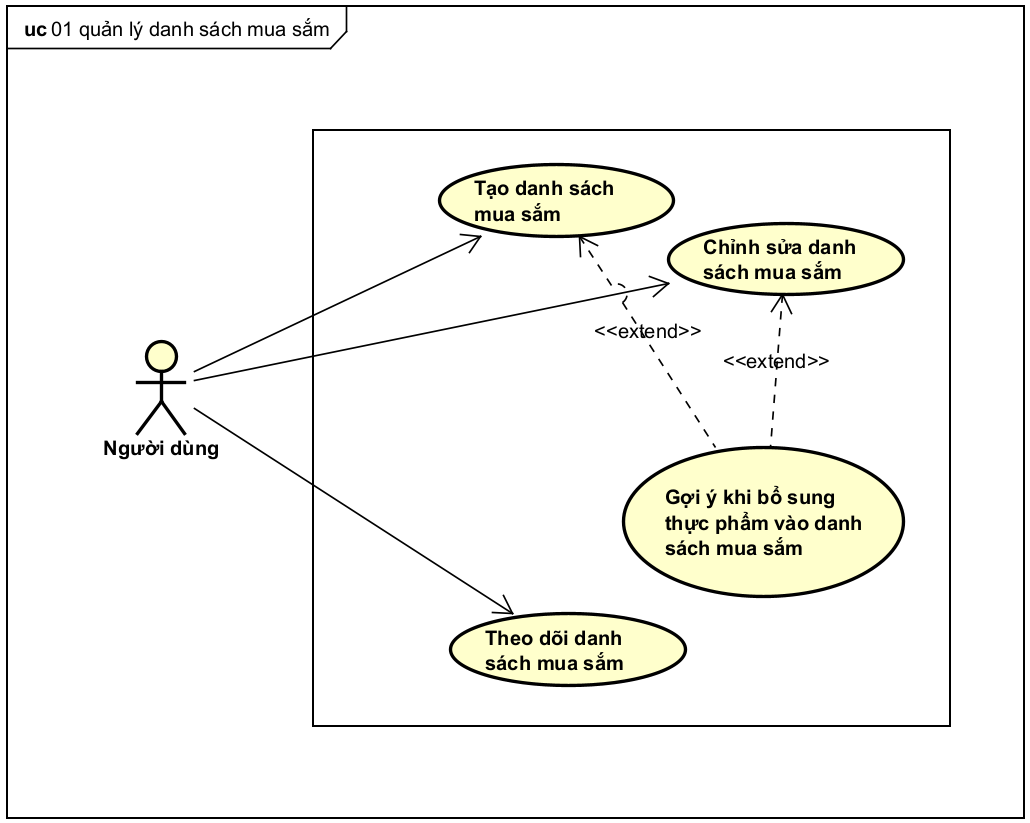
\includegraphics[width=0.9\textwidth]{UC_Danh_sach_mua_sam.png}
    \caption{Biểu đồ Usecase quản lý danh sách mua sắm}
    \label{fig:usecase-01}
\end{figure}

\vspace{1em}

\begin{table}[H]
    \centering
    \label{tab:uc001-1}
    \begin{tabularx}{\textwidth}{|c|p{3.5cm}|X|}
        \hline
        \rowcolor{headergreen} 
        \textbf{Mã UC} & \textbf{UC001.1} & \textbf{Tên UC: Tạo danh sách mua sắm} \\ \hline
        \textbf{Tác nhân} & \multicolumn{2}{l|}{Người dùng} \\ \hline
        \textbf{Điều kiện trước} & \multicolumn{2}{X|}{Người dùng đã tham gia vào một group} \\ \hline
        
        \multicolumn{3}{|c|}{\cellcolor{headerorange}\textbf{Luồng thực thi chính}} \\ \hline
        \rowcolor{graybg} \textbf{STT} & \textbf{Thực hiện} & \textbf{Hành động} \\ \hline
        1 & Người dùng & Điền thực phẩm cần mua \\ \hline
        2 & Người dùng & Chọn người đảm nhận \\ \hline
        3 & Người dùng & Hoàn thành tạo danh sách \\ \hline
        4 & Hệ thống & Lưu vào database \\ \hline
        5 & Hệ thống & Gửi thông báo cho người đảm nhận \\ \hline
        
        \multicolumn{3}{|c|}{\cellcolor{headerorange}\textbf{Luồng thực thi mở rộng}} \\ \hline
        \rowcolor{graybg} \textbf{STT} & \textbf{Thực hiện} & \textbf{Hành động và Điều kiện} \\ \hline
        1a & Hệ thống & \textbf{Điều kiện:} Trong group có thực đơn lên sẵn \newline \textbf{Hành động:} Thực hiện Usecase UC001.4 (Gợi ý bổ sung thực phẩm) \\ \hline
        
        \textbf{Điều kiện sau} & \multicolumn{2}{X|}{Danh sách mua sắm được tạo ra, người đảm nhiệm nhận được thông báo} \\ \hline
    \end{tabularx}
    \caption{Đặc tả ca sử dụng UC001.1: Tạo danh sách mua sắm}
\end{table}

\begin{table}[H]
    \centering
    \label{tab:uc001-3}
    \begin{tabularx}{\textwidth}{|c|p{3.5cm}|X|}
        \hline
        \rowcolor{headergreen} 
        \textbf{Mã UC} & \textbf{UC001.3} & \textbf{Tên UC: Theo dõi danh sách mua sắm} \\ \hline
        \textbf{Tác nhân} & \multicolumn{2}{l|}{Người dùng} \\ \hline
        \textbf{Điều kiện trước} & \multicolumn{2}{X|}{Group đã có danh sách mua sắm tạo trước đó} \\ \hline
        
        \multicolumn{3}{|c|}{\cellcolor{headerorange}\textbf{Luồng thực thi chính}} \\ \hline
        \rowcolor{graybg} \textbf{STT} & \textbf{Thực hiện} & \textbf{Hành động} \\ \hline
        1 & Người dùng & Mở danh sách mua sắm (hiển thị dưới dạng checklist). \\ \hline
        2 & Người dùng & Tick chọn một mặt hàng khi đã mua. \\ \hline
        3 & Hệ thống & Hiển thị hộp thoại nhập số lượng thực tế mua được. \\ \hline
        4 & Người dùng & Nhập số lượng thực tế và xác nhận. \\ \hline
        5 & Hệ thống & Ghi nhận số lượng thực tế đã mua: \newline
        - Nếu số lượng thực tế = số lượng dự định $\rightarrow$ đánh dấu ``đã mua''. \newline
        - Nếu số lượng thực tế < số lượng dự định $\rightarrow$ đánh dấu ``đã mua'' và tạo thêm 1 mục cần mua là số lượng thực phẩm đó còn thiếu. \\ \hline
        6 & Người dùng & Lặp lại cho các mặt hàng khác. \\ \hline
        7 & Người dùng & Chọn hoàn thành đi chợ. \\ \hline
        8 & Người dùng & Gửi thông báo đến toàn group. \\ \hline
        
        \textbf{Điều kiện sau} & \multicolumn{2}{X|}{Thông báo hoàn thành đi chợ được gửi đến toàn group} \\ \hline
    \end{tabularx}
    \caption{Đặc tả ca sử dụng UC001.3: Theo dõi danh sách mua sắm}
\end{table}

\begin{table}[H]
    \centering
    \label{tab:uc001-4}
    \begin{tabularx}{\textwidth}{|c|p{3.5cm}|X|}
        \hline
        \rowcolor{headergreen} 
        \textbf{Mã UC} & \textbf{UC001.4} & \textbf{Tên UC: Gợi ý bổ sung thực phẩm} \\ \hline
        \textbf{Tác nhân} & \multicolumn{2}{l|}{Người dùng} \\ \hline
        \textbf{Điều kiện trước} & \multicolumn{2}{X|}{Người dùng đang cần thêm một mục vào danh sách mua sắm; Trong group của người dùng có ``thực đơn lên sẵn''} \\ \hline
        
        \multicolumn{3}{|c|}{\cellcolor{headerorange}\textbf{Luồng thực thi chính}} \\ \hline
        \rowcolor{graybg} \textbf{STT} & \textbf{Thực hiện} & \textbf{Hành động} \\ \hline
        1 & Hệ thống & Kiểm tra dữ liệu: \newline
        - \textbf{Thực đơn đã lên lịch:} Kiểm tra thực đơn cho những bữa sắp tới. \newline
        - \textbf{Công thức nấu ăn:} Kiểm tra nguyên liệu cần dùng trong thực đơn đó. \newline
        - \textbf{Bếp:} Kiểm tra nguyên liệu đó có trong bếp không. \\ \hline
        2 & Hệ thống & Kiểm tra điều kiện xem nguyên liệu đó có số lượng ít hơn hay khác đơn vị so với công thức hay không. \\ \hline
        3 & Hệ thống & Gợi ý thực phẩm nên bổ sung. \\ \hline
        4 & Người dùng & Chọn đồng ý để thêm thực phẩm vào danh sách mua sắm. \\ \hline
        
        \multicolumn{3}{|c|}{\cellcolor{headerorange}\textbf{Luồng thực thi mở rộng}} \\ \hline
        \rowcolor{graybg} \textbf{STT} & \textbf{Thực hiện} & \textbf{Hành động và Điều kiện} \\ \hline
        2a & Hệ thống & \textbf{Điều kiện:} Nếu thực phẩm đó đã đủ hoặc thừa. \newline
        \textbf{Hành động:} Quay lại bước 1 để tìm nguyên liệu tiếp theo. \\ \hline
        4a & Hệ thống & \textbf{Điều kiện:} Người dùng không đồng ý thêm thực phẩm đó. \newline
        \textbf{Hành động:} Quay lại bước 1 để tìm nguyên liệu tiếp theo. \\ \hline
        
        \textbf{Điều kiện sau} & \multicolumn{2}{X|}{Thực phẩm cần mua được gợi ý cho người dùng} \\ \hline
    \end{tabularx}
    \caption{Đặc tả ca sử dụng UC001.4: Gợi ý khi bổ sung thực phẩm vào danh sách mua sắm}
\end{table}
\textbf{Quản lý dự định bữa ăn }
\begin{figure}[H]
    \centering
    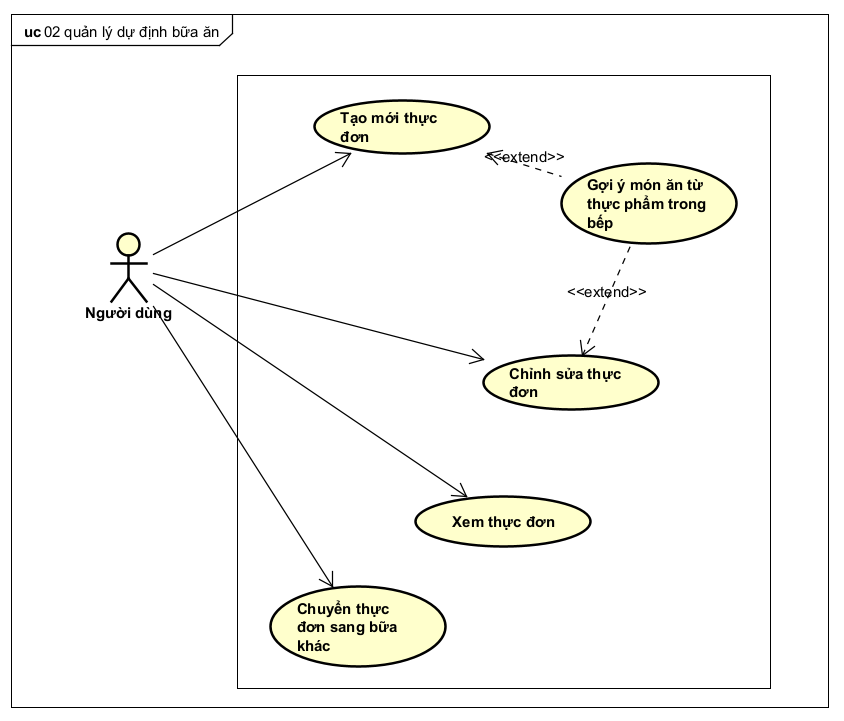
\includegraphics[width=0.9\textwidth]{UC_du_dinh_bua_an.png}
    \caption{Biểu đồ Usecase quản lý dự định bữa ăn}
    \label{fig:usecase-02}
\end{figure}
\begin{table}[H]
    \centering
    \label{tab:uc002-1}
    \begin{tabularx}{\textwidth}{|c|p{3.5cm}|X|}
        \hline
        \rowcolor{headergreen} 
        \textbf{Mã UC} & \textbf{UC002.1} & \textbf{Tên UC: Tạo thực đơn mới} \\ \hline
        \textbf{Tác nhân} & \multicolumn{2}{l|}{Người dùng} \\ \hline
        \textbf{Điều kiện trước} & \multicolumn{2}{X|}{Người dùng đã tham gia vào một group} \\ \hline
        
        \multicolumn{3}{|c|}{\cellcolor{headerorange}\textbf{Luồng thực thi chính}} \\ \hline
        \rowcolor{graybg} \textbf{STT} & \textbf{Thực hiện} & \textbf{Hành động} \\ \hline
        1 & Người dùng & Chọn bữa muốn tạo thực đơn. \\ \hline
        2 & Người dùng & Thêm từng món cho thực đơn. \\ \hline
        3 & Người dùng & Hoàn tất lên thực đơn. \\ \hline
        4 & Hệ thống & Lưu dữ liệu vào database. \\ \hline
        
        \multicolumn{3}{|c|}{\cellcolor{headerorange}\textbf{Luồng thực thi mở rộng}} \\ \hline
        \rowcolor{graybg} \textbf{STT} & \textbf{Thực hiện} & \textbf{Hành động và Điều kiện} \\ \hline
        2a & Hệ thống & \textbf{Điều kiện:} Nếu trong bếp có thực phẩm. \newline
        \textbf{Hành động:} Kích hoạt Usecase UC002.3. \\ \hline
        
        \textbf{Điều kiện sau} & \multicolumn{2}{X|}{Thực đơn mới được tạo ra} \\ \hline
    \end{tabularx}
    \caption{Đặc tả ca sử dụng UC002.1: Tạo thực đơn mới}
\end{table}
\begin{table}[H]
    \centering
    \label{tab:uc002-3}
    \begin{tabularx}{\textwidth}{|c|p{3.5cm}|X|}
        \hline
        \rowcolor{headergreen} 
        \textbf{Mã UC} & \textbf{UC002.3} & \textbf{Tên UC: Gợi ý món ăn từ thực phẩm trong bếp} \\ \hline
        \textbf{Tác nhân} & \multicolumn{2}{l|}{Người dùng} \\ \hline
        \textbf{Điều kiện trước} & \multicolumn{2}{X|}{Người dùng đang thêm món vào thực đơn, trong bếp đã có sẵn thực phẩm} \\ \hline
        
        \multicolumn{3}{|c|}{\cellcolor{headerorange}\textbf{Luồng thực thi chính}} \\ \hline
        \rowcolor{graybg} \textbf{STT} & \textbf{Thực hiện} & \textbf{Hành động} \\ \hline
        1 & Hệ thống & Kiểm tra: \newline
        - \textbf{Bếp:} Kiểm tra các thực phẩm có sẵn trong bếp. \newline
        - \textbf{Thực đơn:} Kiểm tra các món ăn sử dụng thực phẩm đó làm nguyên liệu chính. \\ \hline
        2 & Hệ thống & Gợi ý món ăn đó cho người dùng. \\ \hline
        3 & Người dùng & Đồng ý thêm món vào thực đơn. \\ \hline
        
        \multicolumn{3}{|c|}{\cellcolor{headerorange}\textbf{Luồng thực thi mở rộng}} \\ \hline
        \rowcolor{graybg} \textbf{STT} & \textbf{Thực hiện} & \textbf{Hành động và Điều kiện} \\ \hline
        2a & Hệ thống & \textbf{Điều kiện:} Chọn không đồng ý thêm món ăn. \newline
        \textbf{Hành động:} Quay lại bước 1 để gợi ý món ăn tiếp theo. \\ \hline
        
        \textbf{Điều kiện sau} & \multicolumn{2}{X|}{Thực đơn mới được tạo ra} \\ \hline
    \end{tabularx}
    \caption{Đặc tả ca sử dụng UC002.3: Gợi ý món ăn từ thực phẩm trong bếp}
\end{table}
\textbf{Quản lý thực phẩm trong bếp}
\begin{figure}[H]
    \centering 
    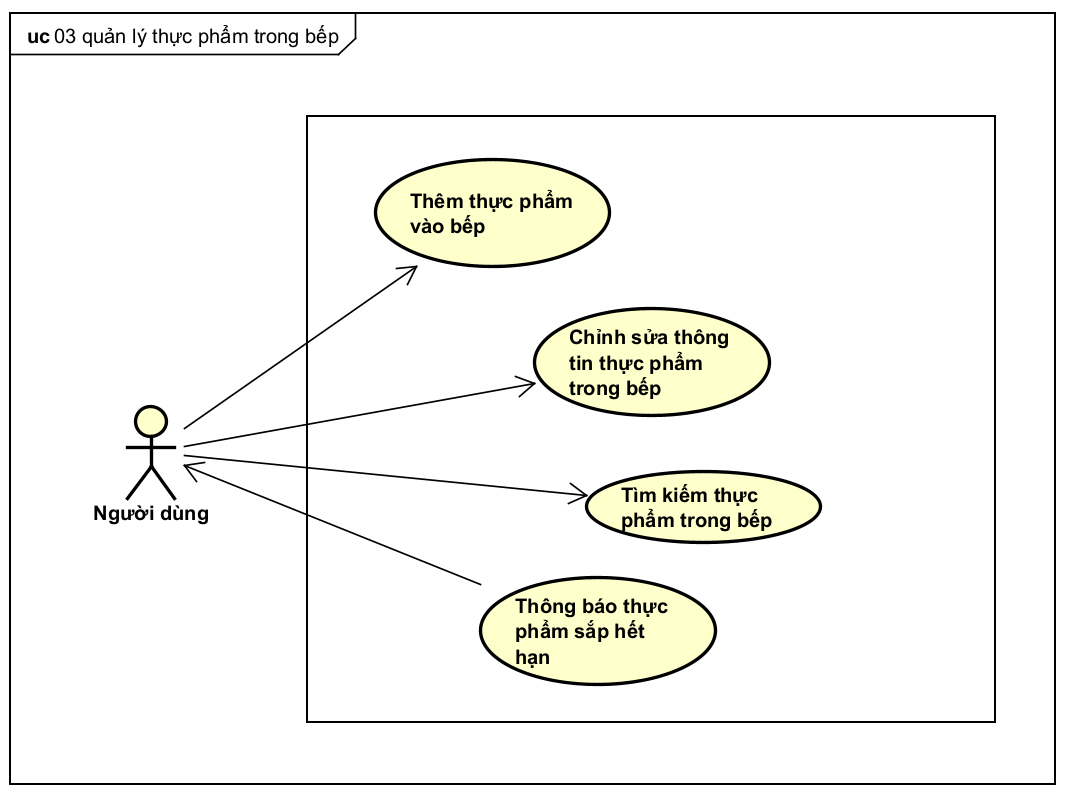
\includegraphics[width=0.9\textwidth]{UC_quan_ly_thucpham_trongbep.png}
    \caption{Biểu đồ Use Case quản lý thực phẩm trong bếp}
    \label{fig:usecase-03}
\end{figure}

\begin{table}[H]
    \centering
    \label{tab:uc003-1}
    \begin{tabularx}{\textwidth}{|c|p{3.5cm}|X|}
        \hline
        \rowcolor{headergreen} 
        \textbf{Mã UC} & \textbf{UC003.1} & \textbf{Tên UC: Thêm thực phẩm vào bếp} \\ \hline
        \textbf{Tác nhân} & \multicolumn{2}{l|}{Người dùng} \\ \hline
        \textbf{Điều kiện trước} & \multicolumn{2}{X|}{Người dùng đã tham gia vào một group} \\ \hline
        
        \multicolumn{3}{|c|}{\cellcolor{headerorange}\textbf{Luồng thực thi chính}} \\ \hline
        \rowcolor{graybg} \textbf{STT} & \textbf{Thực hiện} & \textbf{Hành động} \\ \hline
        1 & Người dùng & Chọn thêm thực phẩm. \\ \hline
        2 & Người dùng & Điền thông tin thực phẩm. \\ \hline
        3 & Hệ thống & Lưu dữ liệu vào database. \\ \hline
        
        \multicolumn{3}{|c|}{\cellcolor{headerorange}\textbf{Luồng thực thi mở rộng}} \\ \hline
        \rowcolor{graybg} \textbf{STT} & \textbf{Thực hiện} & \textbf{Hành động và Điều kiện} \\ \hline
        2a & Hệ thống & \textbf{Điều kiện:} Nếu trong bếp có thực phẩm. \newline
        \textbf{Hành động:} Kích hoạt Usecase UC002.3. \\ \hline
        
        \textbf{Điều kiện sau} & \multicolumn{2}{X|}{Thực phẩm mới được thêm vào trong bếp} \\ \hline
    \end{tabularx}
    \caption{Đặc tả ca sử dụng UC003.1: Thêm thực phẩm vào bếp}
\end{table}
\begin{table}[H]
    \centering
    \label{tab:uc003-2}
    \begin{tabularx}{\textwidth}{|c|p{3.5cm}|X|}
        \hline
        \rowcolor{headergreen} 
        \textbf{Mã UC} & \textbf{UC003.2} & \textbf{Tên UC: Chỉnh sửa thực phẩm trong bếp} \\ \hline
        \textbf{Tác nhân} & \multicolumn{2}{l|}{Người dùng} \\ \hline
        \textbf{Điều kiện trước} & \multicolumn{2}{X|}{Trong tủ lạnh đã có sẵn sản phẩm} \\ \hline
        
        \multicolumn{3}{|c|}{\cellcolor{headerorange}\textbf{Luồng thực thi chính}} \\ \hline
        \rowcolor{graybg} \textbf{STT} & \textbf{Thực hiện} & \textbf{Hành động} \\ \hline
        1 & Người dùng & Chọn thực phẩm cần chỉnh sửa. \\ \hline
        2 & Người dùng & Chỉnh sửa thông tin thực phẩm (Chỉ chỉnh sửa số lượng và đơn vị). \\ \hline
        3 & Hệ thống & Lưu dữ liệu vào database. \\ \hline
        
        \textbf{Điều kiện sau} & \multicolumn{2}{X|}{Thực phẩm được chỉnh sửa ở danh sách thực phẩm trong bếp} \\ \hline
    \end{tabularx}
    \caption{Đặc tả ca sử dụng UC003.2: Chỉnh sửa thực phẩm trong bếp}
\end{table}
\textbf{Quản lý công thức nấu ăn}
\begin{figure}[H]
    \centering 
    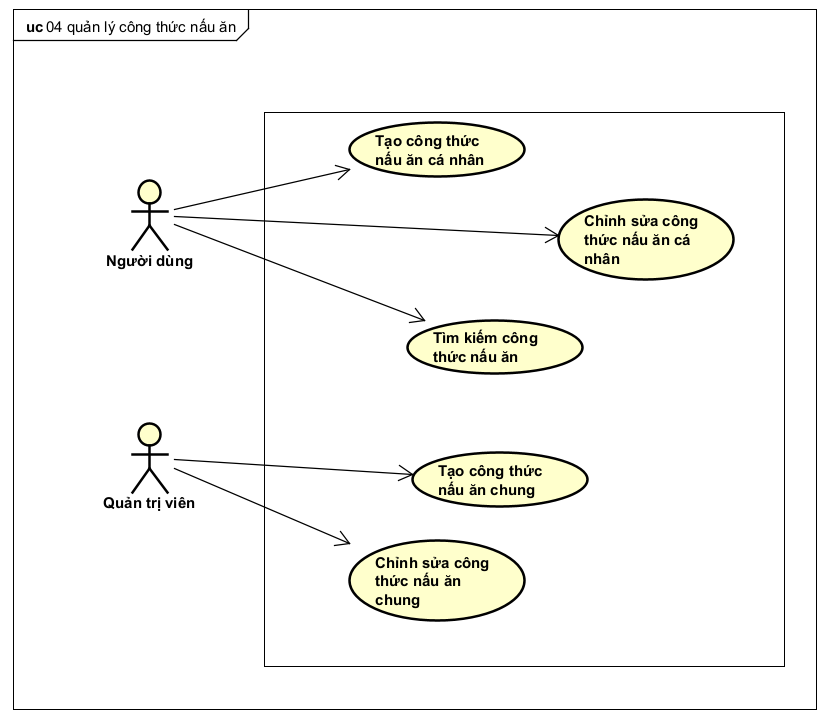
\includegraphics[width=0.9\textwidth]{UC_Quanly_congthuc.png}
    \caption{Biểu đồ Use Case quản lý công thức nấu ăn}
    \label{fig:usecase-04}
\end{figure}
\begin{table}[H]
    \centering
    \label{tab:uc004-1}
    \begin{tabularx}{\textwidth}{|c|p{3.5cm}|X|}
        \hline
        \rowcolor{headergreen} 
        \textbf{Mã UC} & \textbf{UC004.1} & \textbf{Tên UC: Tạo công thức nấu ăn chung} \\ \hline
        \textbf{Tác nhân} & \multicolumn{2}{l|}{Quản trị viên} \\ \hline
        \textbf{Điều kiện trước} & \multicolumn{2}{X|}{Quản trị viên đã đăng nhập} \\ \hline
        
        \multicolumn{3}{|c|}{\cellcolor{headerorange}\textbf{Luồng thực thi chính}} \\ \hline
        \rowcolor{graybg} \textbf{STT} & \textbf{Thực hiện} & \textbf{Hành động} \\ \hline
        1 & Quản trị viên & Chọn tạo công thức nấu ăn chung. \\ \hline
        2 & Quản trị viên & Điền thông tin cho công thức nấu ăn mới. \\ \hline
        3 & Quản trị viên & Hoàn thành điền thông tin. \\ \hline
        4 & Hệ thống & Lưu dữ liệu vào database. \\ \hline
        
        \textbf{Điều kiện sau} & \multicolumn{2}{X|}{Công thức nấu ăn chung mới được tạo ra} \\ \hline
    \end{tabularx}
    \caption{Đặc tả ca sử dụng UC004.1: Tạo công thức nấu ăn chung}
\end{table}
\begin{table}[H]
    \centering
    \label{tab:uc004-3}
    \begin{tabularx}{\textwidth}{|c|p{3.5cm}|X|}
        \hline
        \rowcolor{headergreen} 
        \textbf{Mã UC} & \textbf{UC004.3} & \textbf{Tên UC: Tạo công thức nấu ăn cá nhân} \\ \hline
        \textbf{Tác nhân} & \multicolumn{2}{l|}{Người dùng} \\ \hline
        \textbf{Điều kiện trước} & \multicolumn{2}{X|}{Người dùng đã tham gia vào nhóm} \\ \hline
        
        \multicolumn{3}{|c|}{\cellcolor{headerorange}\textbf{Luồng thực thi chính}} \\ \hline
        \rowcolor{graybg} \textbf{STT} & \textbf{Thực hiện} & \textbf{Hành động} \\ \hline
        1 & Người dùng & Chọn tạo công thức nấu ăn cho nhóm. \\ \hline
        2 & Người dùng & Điền thông tin cho công thức nấu ăn mới. \\ \hline
        3 & Người dùng & Hoàn thành điền thông tin. \\ \hline
        4 & Hệ thống & Lưu dữ liệu vào database. \\ \hline
        
        \textbf{Điều kiện sau} & \multicolumn{2}{X|}{Công thức nấu ăn cá nhân mới được tạo ra} \\ \hline
    \end{tabularx}
    \caption{Đặc tả ca sử dụng UC004.3: Tạo công thức nấu ăn cá nhân}
\end{table}
\begin{table}[H]
    \centering
    \label{tab:uc004-5}
    \begin{tabularx}{\textwidth}{|c|p{3.5cm}|X|}
        \hline
        \rowcolor{headergreen} 
        \textbf{Mã UC} & \textbf{UC004.5} & \textbf{Tên UC: Tìm kiếm công thức món ăn} \\ \hline
        \textbf{Tác nhân} & \multicolumn{2}{l|}{Người dùng} \\ \hline
        \textbf{Điều kiện trước} & \multicolumn{2}{X|}{Người dùng đã đăng nhập} \\ \hline
        
        \multicolumn{3}{|c|}{\cellcolor{headerorange}\textbf{Luồng thực thi chính}} \\ \hline
        \rowcolor{graybg} \textbf{STT} & \textbf{Thực hiện} & \textbf{Hành động} \\ \hline
        1 & Người dùng & Nhập vào thanh tìm kiếm tên món ăn hoặc nguyên liệu. \\ \hline
        2 & Hệ thống & Trả về danh sách món ăn. \\ \hline
        
        \textbf{Điều kiện sau} & \multicolumn{2}{X|}{Trả về danh sách kết quả các món ăn} \\ \hline
    \end{tabularx}
    \caption{Đặc tả ca sử dụng UC004.5: Tìm kiếm công thức món ăn}
\end{table}
\textbf{Quản lý danh sách thực phẩm}
\begin{figure}[H]
    \centering 
    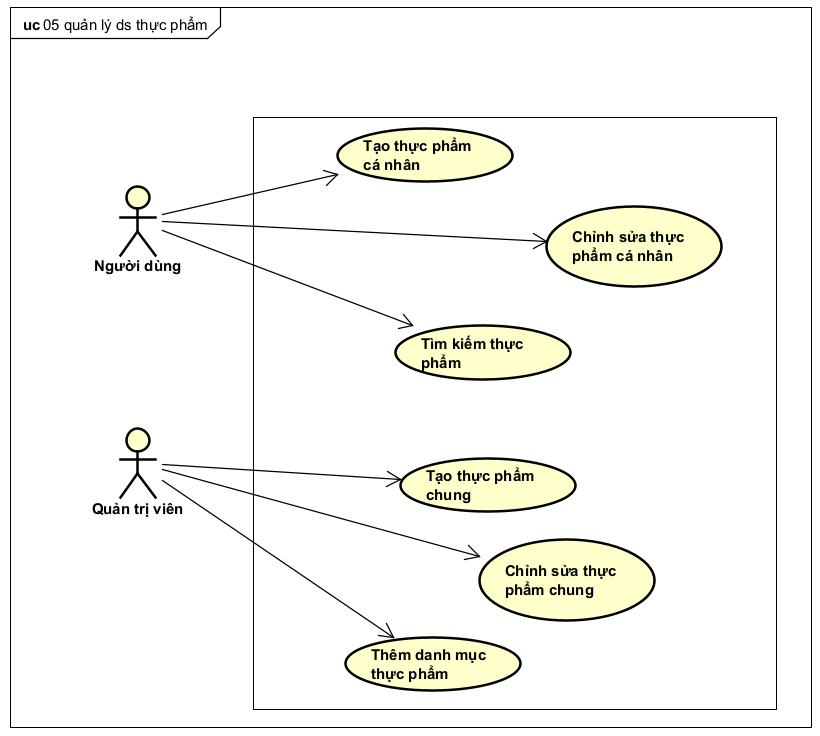
\includegraphics[width=0.9\textwidth]{UC_Quanly_danhsach_thucpham.png}
    \caption{Biểu đồ Use Case quản lý danh sách thực phẩm}
    \label{fig:usecase-05}
\end{figure}
\begin{table}[H]
    \centering
    \label{tab:uc005-1}
    \begin{tabularx}{\textwidth}{|c|p{3.5cm}|X|}
        \hline
        \rowcolor{headergreen} 
        \textbf{Mã UC} & \textbf{UC005.1} & \textbf{Tên UC: Tạo thực phẩm cá nhân} \\ \hline
        \textbf{Tác nhân} & \multicolumn{2}{l|}{Người dùng} \\ \hline
        \textbf{Điều kiện trước} & \multicolumn{2}{X|}{Người dùng đã tham gia vào nhóm} \\ \hline
        
        \multicolumn{3}{|c|}{\cellcolor{headerorange}\textbf{Luồng thực thi chính}} \\ \hline
        \rowcolor{graybg} \textbf{STT} & \textbf{Thực hiện} & \textbf{Hành động} \\ \hline
        1 & Người dùng & Chọn thực phẩm mới cho nhóm. \\ \hline
        2 & Người dùng & Điền thông tin cho thực phẩm mới. \\ \hline
        3 & Hệ thống & Kiểm tra tên thực phẩm có trùng không. \\ \hline
        4 & Người dùng & Hoàn thành tạo thực phẩm mới. \\ \hline
        5 & Hệ thống & Lưu dữ liệu vào database. \\ \hline
        
        \textbf{Điều kiện sau} & \multicolumn{2}{X|}{Thực phẩm cá nhân mới được tạo ra} \\ \hline
    \end{tabularx}
    \caption{Đặc tả ca sử dụng UC005.1: Tạo thực phẩm cá nhân}
\end{table}
\textbf{Quản lý nhóm}
\begin{figure}[H]
    \centering 
    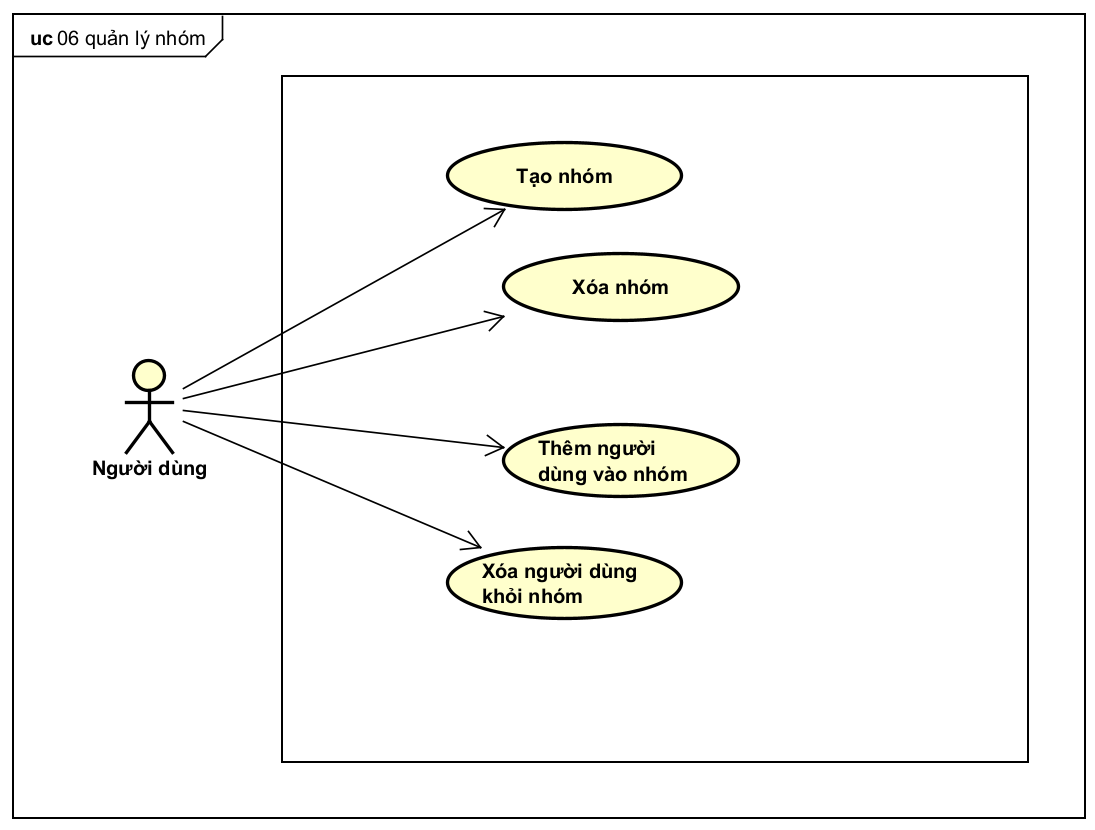
\includegraphics[width=0.9\textwidth]{UC_quanly_nhom.png}
    \caption{Biểu đồ Use Case quản lý nhóm}
    \label{fig:usecase-06}
\end{figure}
\textbf{Quản trị người dùng}
\begin{figure}[H]
    \centering 
    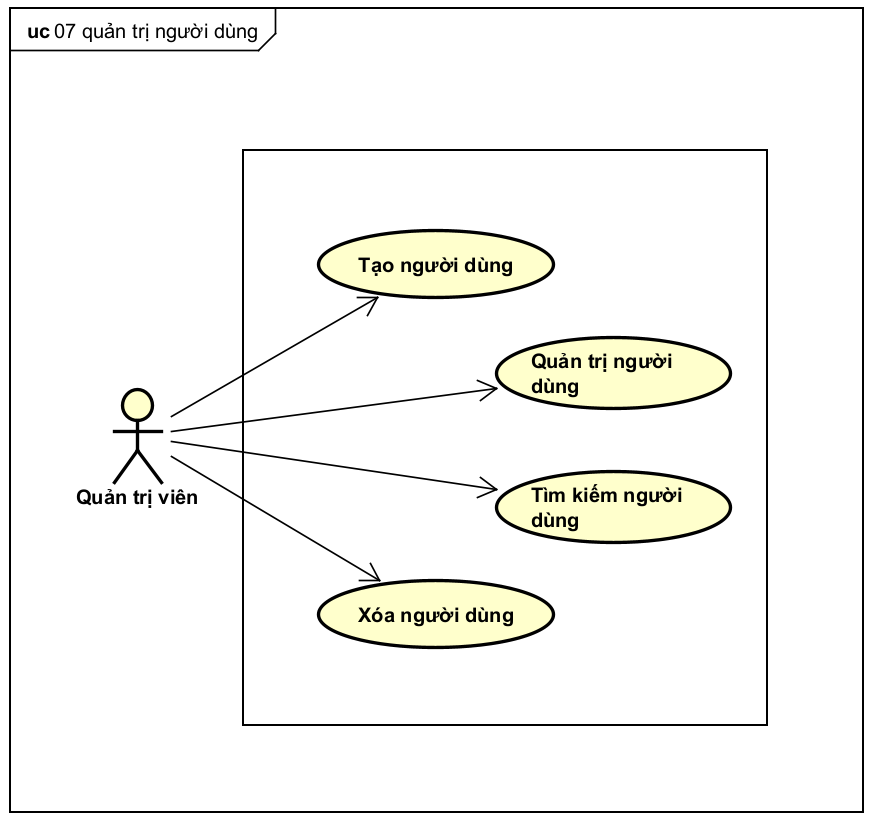
\includegraphics[width=0.9\textwidth]{UC_quanly_nguoidung.png}
    \caption{Biểu đồ Use Case quản lý người dùng}
    \label{fig:usecase-07}
\end{figure}
\subsection{Các yêu cầu phi chức năng}
\subsubsection{Tính dễ dùng}
\begin{itemize}
    \item Giao diện người dùng được thiết kế thân thiện, dễ hiểu, sử dụng được cho cả người dùng ít kinh nghiệm với công nghệ.
    \item Các thao tác như tạo, chỉnh sửa, xóa dữ liệu cần rõ ràng và có xác nhận trước khi thực hiện.
    \item Khi người dùng nhập sai dữ liệu, hệ thống phải hiển thị thông báo lỗi cụ thể, dễ hiểu, gồm:
    \begin{itemize}
        \item Mô tả lỗi (``Ngày hết hạn không hợp lệ'').
        \item Gợi ý cách khắc phục (``Vui lòng nhập ngày hợp lệ theo định dạng DD/MM/YYYY'').
    \end{itemize}
    \item Các biểu tượng và nút bấm có chú thích, gợi ý (tooltip, placeholder).
    \item Màu sắc, kích thước chữ, bố cục cần đảm bảo tính dễ đọc và nhất quán trên nhiều thiết bị (điện thoại, máy tính bảng).
\end{itemize}

\subsubsection{Hiệu năng}
\begin{itemize}
    \item Ứng dụng cần phản hồi các thao tác người dùng trong vòng 2 giây cho các chức năng cơ bản (tạo, sửa, xem danh sách, tìm kiếm).
    \item Tốc độ tải dữ liệu từ server phải đảm bảo mượt mà, không gây giật lag trong quá trình sử dụng.
    \item Cơ chế cache cục bộ được sử dụng để truy cập nhanh dữ liệu gần nhất khi thiết bị mất kết nối Internet.
    \item Hệ thống backend (server và CSDL) cần hỗ trợ tối thiểu 1000 người dùng đồng thời trong giai đoạn triển khai thử nghiệm.
\end{itemize}

\subsubsection{Tính tin cậy}
\begin{itemize}
    \item Hệ thống phải lưu trữ dữ liệu an toàn, không bị mất khi người dùng tắt ứng dụng đột ngột hoặc mất mạng.
    \item Dữ liệu người dùng được đồng bộ lên server ngay khi có kết nối mạng trở lại.
    \item Cơ chế sao lưu (backup) dữ liệu định kỳ mỗi ngày.
    \item Tự động phục hồi (auto-reconnect) khi mất kết nối ngắn hạn.
\end{itemize}

\subsubsection{Tính dễ bảo trì}
\begin{itemize}
    \item Mã nguồn được chia thành các module rõ ràng: frontend (giao diện), backend (API, xử lý logic), database (lưu trữ).
    \item Có tài liệu hướng dẫn cài đặt, cấu hình, và hướng dẫn lập trình viên mở rộng chức năng.
    \item Hệ thống được phát triển theo mô hình RESTful API, dễ dàng thay đổi hoặc mở rộng sang các nền tảng khác (web, desktop).
    \item Sử dụng công nghệ phổ biến, mã nguồn mở để dễ dàng bảo trì, cập nhật phiên bản.
\end{itemize}

\subsubsection{Tính khả chuyển}
\begin{itemize}
    \item Ứng dụng được phát triển bằng công nghệ đa nền tảng (ví dụ: Flutter hoặc React Native), có thể chạy trên cả Android và iOS.
    \item Cấu hình hệ thống linh hoạt, dễ dàng triển khai trên nhiều môi trường (local, cloud).
    \item Dữ liệu được lưu trữ trên cơ sở dữ liệu đám mây (ví dụ: Firebase, MongoDB Atlas hoặc MySQL Cloud).
\end{itemize}

\subsubsection{Yêu cầu an toàn bảo mật}
\begin{itemize}
    \item Dữ liệu người dùng được mã hóa khi truyền giữa client và server (sử dụng HTTPS).
    \item Mật khẩu người dùng phải được lưu trữ dưới dạng mã hóa (hash + salt).
    \item Mỗi tài khoản người dùng chỉ được phép truy cập và chỉnh sửa dữ liệu cá nhân hoặc dữ liệu nhóm mà họ thuộc về.
    \item Cơ chế phân quyền rõ ràng: người dùng, trưởng nhóm gia đình, quản trị viên.
    \item Hạn chế truy cập trái phép qua API (sử dụng JWT token hoặc OAuth2).
\end{itemize}

\subsubsection{Yêu cầu về giao diện}
\begin{itemize}
    \item Giao diện người dùng (UI) được thiết kế theo phong cách tối giản, hiện đại, hỗ trợ chế độ Dark/Light mode.
    \item Có màn hình hướng dẫn sử dụng (onboarding) cho người dùng mới.
    \item Toàn bộ giao diện phải hiển thị tốt trên màn hình từ 5--10 inch (smartphone, tablet).
    \item Các biểu tượng, màu sắc và font chữ thống nhất với bộ nhận diện thương hiệu của ứng dụng.
\end{itemize}

\newpage
\section{Thiết kế giao diện}
\subsection{Thiết kế giao diện low-fidelity / mid-fidelity prototype}
\subsection{Xây dựng các màn hình giao diện của ứng dụng (high-fidelity)}
\newpage
\section{Thiết kế Backend}
\subsection{Thiết kế cơ sở dữ liệu cho Backend}
\subsection{Thiết kế API Backend}
\subsubsection{Danh sách API}
\subsubsection{Đặc tả chi tiết API}


\newpage
\section{Xây dựng ứng dụng đa nền tảng}
\subsection{Kiến trúc ứng dụng}

\subsubsection{Lựa chọn kiến trúc phần mềm và giải thích sơ bộ}

Ứng dụng \textbf{``Đi chợ tiện lợi''} được xây dựng theo mô hình \textbf{Client-Server Architecture} kết hợp với \textbf{RESTful API}, trong đó:

\begin{itemize}
    \item \textbf{Client (Frontend):} Ứng dụng di động đa nền tảng phát triển bằng React Native + Expo.
    \item \textbf{Server (Backend):} Hệ thống API server xây dựng bằng Spring Boot (Java).
    \item \textbf{Database:} PostgreSQL để lưu trữ dữ liệu.
\end{itemize}

\paragraph{Kiến trúc Backend: Clean Architecture}
Phía Backend được thiết kế theo \textbf{Clean Architecture} với nguyên tắc \textbf{Dependency Inversion} - các lớp bên trong không phụ thuộc vào các lớp bên ngoài. Các đặc điểm chính:
\begin{itemize}
    \item \textbf{Độc lập với Framework:} Logic nghiệp vụ không phụ thuộc vào framework cụ thể.
    \item \textbf{Có thể kiểm thử (Testable):} Business logic có thể test độc lập.
    \item \textbf{Độc lập với Database:} Có thể thay đổi database mà không ảnh hưởng nghiệp vụ.
\end{itemize}

\paragraph{Kiến trúc Frontend: Component-Based Architecture}
Phía Frontend sử dụng \textbf{Component-Based Architecture} kết hợp với \textbf{React Query} cho server state và \textbf{Zustand} cho client state:
\begin{itemize}
    \item \textbf{Component-Based:} Giao diện được chia thành các component độc lập, tái sử dụng.
    \item \textbf{Unidirectional Data Flow:} Luồng dữ liệu một chiều với State Management.
\end{itemize}

\subsubsection{Các cải tiến so với lý thuyết}

\begin{enumerate}
    \item \textbf{Tách biệt JPA Entity và Domain Entity:} Domain Entity là pure Java object, JPA Model chứa các annotations. Mapper class chịu trách nhiệm chuyển đổi qua lại, giúp lõi nghiệp vụ hoàn toàn sạch (clean).
    \item \textbf{Use Case Pattern:} Thay vì một Service class khổng lồ, mỗi UseCase tập trung vào một nhóm chức năng cụ thể, giúp tuân thủ nguyên tắc Single Responsibility.
    \item \textbf{Repository Pattern với Interface Segregation:} Domain layer định nghĩa interface, Infrastructure layer triển khai thực tế. Điều này cho phép dễ dàng thay đổi công nghệ lưu trữ (ví dụ từ SQL sang NoSQL) mà không sửa đổi logic nghiệp vụ.
    \item \textbf{React Query cho Server State:} Thay vì quản lý mọi thứ trong Global State (như Redux), ứng dụng dùng React Query để tối ưu hóa việc caching, đồng bộ dữ liệu và giảm thiểu số lượng API call không cần thiết.
\end{enumerate}

\subsection{Tổ chức thư mục của dự án}
\subsection{Thiết kế chi tiết các gói}
\subsection{Thiết kế chi tiết lớp}
\subsection{Các giải pháp khác đã xây dựng trong chương trình}

\newpage
\section{Kiểm thử chương trình}
\subsection{Kiểm thử các chức năng đã thực hiện}
\subsection{Kiểm thử yêu cầu phi chức năng}

\section*{KẾT LUẬN VÀ HƯỚNG PHÁT TRIỂN}
Trong khuôn khổ học phần \textbf{IT4788 - Phát triển ứng dụng đa nền tảng}, dự án xây dựng ứng dụng \textbf{FreshFridge - ``Đi chợ tiện lợi''} đã hoàn thành các mục tiêu đề ra về việc tạo ra một giải pháp quản lý thực phẩm và mua sắm thông minh. Dưới đây là những tổng kết chi tiết về quá trình thực hiện và lộ trình cải tiến hệ thống trong tương lai.

\subsection*{1. Kết luận}

\subsubsection*{1.1. Những kết quả đã đạt được}
Dự án đã hiện thực hóa thành công một hệ thống quản lý tích hợp với các kết quả cụ thể sau:
\begin{itemize}
    \item \textbf{Về chức năng:} Hoàn thiện các module cốt lõi bao gồm: quản lý kho thực phẩm (theo dõi vị trí, số lượng, hạn sử dụng), danh sách mua sắm nhóm, kế hoạch bữa ăn và hệ thống thông báo đẩy (Push Notifications) nhắc nhở thông minh.
    \item \textbf{Về kỹ thuật:} Xây dựng hệ thống ổn định dựa trên kiến trúc \textbf{Clean Architecture} (Back-end Spring Boot) và kiến trúc \textbf{Component-based} (Front-end React Native + Expo). Hệ thống đảm bảo tính nhất quán dữ liệu thông qua PostgreSQL và khả năng đồng bộ thời gian thực với React Query.
    \item \textbf{Về bảo mật và lưu trữ:} Triển khai cơ chế xác thực JWT, mã hóa dữ liệu nhạy cảm trên thiết bị (Secure Store) và tối ưu hóa hình ảnh qua Cloudinary.
\end{itemize}

\subsubsection*{1.2. Ưu điểm và hạn chế}
\begin{itemize}
    \item \textbf{Ưu điểm:} Ứng dụng có giao diện thân thiện, tính thực tiễn cao trong việc giải quyết bài toán lãng phí thực phẩm. Cấu trúc mã nguồn được tổ chức chặt chẽ, sử dụng TypeScript giúp giảm thiểu lỗi runtime và dễ dàng bảo trì.
    \item \textbf{Hạn chế:} Hệ thống chưa triển khai cơ chế Caching (Redis) để tối ưu hóa hiệu năng API. Ngoài ra, việc thiếu kiểm thử tự động (E2E Testing) và các tính năng thông minh dựa trên AI/ML là những điểm cần được khắc phục trong các phiên bản tiếp theo.
\end{itemize}



\subsection*{2. Hướng phát triển}

Dựa trên những hạn chế đã nêu, lộ trình phát triển của FreshFridge được định hướng theo ba giai đoạn:

\subsubsection*{2.1. Ngắn hạn: Tối ưu hóa và Bảo mật}
\begin{itemize}
    \item Triển khai \textbf{Redis Caching} và tối ưu hóa truy vấn cơ sở dữ liệu để nâng cao tốc độ phản hồi.
    \item Tăng tỷ lệ bao phủ kiểm thử (Unit Test \& Integration Test) lên trên 80\%.
    \item Bổ sung cơ chế bảo mật nâng cao như \textbf{Refresh Token Rotation} và \textbf{Rate Limiting} để bảo vệ tài nguyên hệ thống.
\end{itemize}

\subsubsection*{2.2. Trung hạn: Tính năng thông minh và Đa ngữ}
\begin{itemize}
    \item Tích hợp \textbf{Barcode Scanner} và công nghệ \textbf{OCR} để hỗ trợ người dùng nhập liệu thực phẩm từ hóa đơn hoặc mã vạch sản phẩm.
    \item Xây dựng mô hình \textbf{AI Suggestion} để đề xuất món ăn dựa trên nguyên liệu thực tế và thói quen dinh dưỡng của người dùng.
    \item Hoàn thiện hệ thống đa ngôn ngữ (Internationalization) để tiếp cận người dùng quốc tế.
\end{itemize}

\subsubsection*{2.3. Dài hạn: Hệ sinh thái IoT và Cộng đồng}
\begin{itemize}
    \item Kết nối với các thiết bị \textbf{Smart Fridge} và các thiết bị gia dụng IoT để tự động hóa quy trình kiểm kê thực phẩm.
    \item Phát triển mạng xã hội chia sẻ công thức nấu ăn và các giải pháp quản lý chi tiêu thực phẩm dành cho doanh nghiệp nhỏ (nhà hàng, canteen).
    \item Triển khai hệ thống trên hạ tầng đám mây chuyên nghiệp với quy trình \textbf{CI/CD} và giám sát tập trung (ELK Stack).
\end{itemize}

\subsection*{3. Tổng kết cuối cùng}
Ứng dụng FreshFridge không chỉ là một sản phẩm kỹ thuật mà còn là giải pháp thực tế hướng tới lối sống hiện đại và bền vững. Với nền tảng kiến trúc hiện có, hệ thống hoàn toàn đủ tiềm năng để mở rộng thành một hệ sinh thái quản lý gia đình thông minh, mang lại giá trị thiết thực cho cộng đồng người dùng.
\section*{Tài liệu tham khảo}
\addcontentsline{toc}{section}{Tài liệu tham khảo} % Để hiện thị trong mục lục

\begin{enumerate}[label={[\arabic*]}] % Định dạng [1], [2], ...
    % Sách/Giáo trình
    \item \textit{Bài giảng môn Phát triển ứng dụng đa nền tảng}, Đại học Bách Khoa Hà Nội.

    \item Spring Projects, ``Spring Boot Documentation'', \textit{Spring.io}. 
    
    \url{https://docs.spring.io/spring-boot/index.html}.

    \item Meta Platforms, Inc., ``Learn React Native'', \textit{reactnative.dev}. 
    
    \url{https://reactnative.dev/}.
\end{enumerate}
\section*{Phụ lục}
\addcontentsline{toc}{section}{Phụ lục}

\begin{enumerate}
    \item \textbf{Mã nguồn dự án (Github Repository):} \\
    \url{https://github.com/ntabodoiqua/cnweb_20251}

    \item \textbf{Tài liệu báo cáo, Slide và Demo:} \\
    \url{https://drive.google.com/drive/folders/1MyE1HaZQWU9Q3x9vgnKUuMEbEk0ISfUe?usp=sharing}

    \item \textbf{Địa chỉ website dự án:} \\
    \url{https://nguyentheanh-nta.id.vn/}
    \begin{itemize}
        \item \textit{Tài khoản Admin:} \texttt{admin} / \texttt{admin}
    \end{itemize}

    \item \textbf{Hệ thống giám sát (Grafana):} \\
    \url{https://nguyentheanh-nta.id.vn/monitor/}
    \begin{itemize}
        \item \textit{Tài khoản monitor:} \texttt{admin} / \texttt{Theanh@3007}
    \end{itemize}

    \item \textbf{Jira và Github Contributions}
\end{enumerate}



\end{document}
